Training distributions often do not cover all of the test distributions we would like a supervised classifier or model to perform well on.
Often, this is caused by biased dataset collection \citep{torralba2011unbiased} or test distribution drift over time \citep{quionera2009dataset}.
Therefore, a key challenge in training machine learning models in these settings is ensuring they are robust to unseen examples. %without access to the full underlying distribution.
Since it is impossible to generalize to the entire distribution, methods often focus on the adjacent goal of \textit{out-of-domain robustness}.

Data augmentation is a common technique used to improve out-of-domain (OOD) robustness by synthetically generating new training examples \citep{Simard1998}, often by perturbing existing examples in the input space \citep{perez2017}. 
If data concentrates on a low-dimensional manifold \citep{chapelle2006semi}, then these synthetic examples should lie in a manifold neighborhood of the original examples \citep{vicinal200olivier}.
Training models to be robust to such local perturbations has been shown to be effective in improving performance and generalization in semi-supervised and self-supervised settings \citep{bachman2014learning,szegedy2014intriguing, sajjadi2016regularization}.
When the underlying data manifold exhibits easy-to-characterize properties, as in natural images, simple transformations such as translation and rotation %for natural images 
%VP: I think you are using "underlying data manifold [which] exhibit easy-to-characterize properties" to contrast with language (which doesn't have these properties). But to me it isn't a self-evident contrast. Maybe having like "When the underlying data manifold exhibits easy-to-characterise properties as with natural images" or something makes the contrast more obvious?
can quickly generate local training examples.
However, in domains such as natural language, it is much more difficult to find a set of invariances that preserves meaning or semantics.

\begin{figure}[t!]
\centering
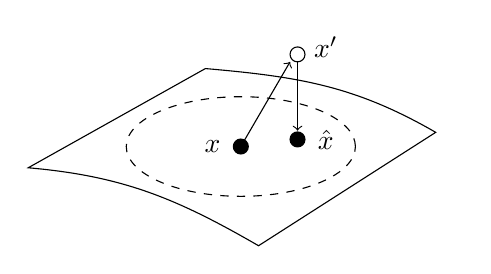
\begin{tikzpicture}[scale=0.9]

% we draw the surface
\draw (0,0) to[out=-5,in=150] (3.25,-1.1) -- (5.75,0.5) to[out=150,in=-5] (2.5,1.4) -- cycle;
\node at (6, 1) {$\M$};

% orginal point
\coordinate (x) at (3.0, 0.3);
\draw[fill] (x) circle (3pt);
\node at (2.6, 0.3) {$x$};

% perturbed point
\coordinate (qx) at (3.8, 1.6);
\draw (qx) circle (3pt);
\node at (4.2, 1.7) {$x'$};

% reconstructed point
\coordinate(rqx) at (3.8, 0.4);
\draw[fill] (rqx) circle (3pt);
\node at (4.2, 0.4) {$\hat{x}$};

\draw [dashed] (x) ellipse (46pt and 20pt);

\draw [->] (x) -- ([xshift=-3pt,yshift=-3pt]qx);
\draw [->] ([yshift=-3pt]qx) -- ([yshift=3.5pt]rqx);
%\draw [->] (x) -- ([xshift=-3.5pt]rqx);
\end{tikzpicture}
\caption{\ssmba\ moves along the data manifold $\M$ by using a corruption function to perturb an example $x$ off the data manifold, then using 
a reconstruction function to project it back on.}
\label{fig:ssmba_process}
\end{figure}
%%%%%%%%%%%%%%%%%%%%%%%%%%%%%%%%%%%%%%%%%%


In this paper we propose \textbf{S}elf-\textbf{S}upervised \textbf{M}anifold \textbf{B}ased Data \textbf{A}ugmentation (\textbf{\ssmba}): a data augmentation method for generating synthetic examples in domains where the data manifold is difficult to heuristically characterize.
Motivated by the use of denoising auto-encoders as generative models \citep{bengio2013generalized}, we use a corruption function to stochastically perturb examples \textit{off} the data manifold, then use a reconstruction function to project them \textit{back on} (Figure \ref{fig:ssmba_process}).
This ensures new examples lie within the manifold neighborhood of the original example.
SSMBA is applicable to any supervised task, requires no task-specific knowledge, and does not rely on class- or dataset-specific fine-tuning.

We investigate the use of \ssmba\ in the natural language domain on 3 diverse tasks spanning both classification and sequence modelling: sentiment analysis, natural language inference, and machine translation.
In experiments across 9 datasets and 4 model types, we show \ssmba\ consistently outperforms baseline models and other data augmentation methods on both in-domain and OOD data. % including Easy Data Augmentation (EDA) \citep{wei-zou-2019-eda}, Conditional BERT Contextual Augmentation (CBERT) \citep{wu2019conditional}, and Unsupervised Data Augmentation (UDA) \citep{xie2020unsupervised}, on both OOD and in-domain (ID) data. 
